\section{Exceptional prolongation: from dodecaphasic incidence to Moonshine}
\label{exc:seccion}

The numerical expression does not exhaust the state that generated it. In the
preceding construction, APP preserves both sheets and division with
remainder and quotient; the TRIT determines the local regime and its orientation;
the TPK composes selection, transport, carry, memory, and return. The
Archimedean readout contracts compatible cylinders. The readout that we now
study instead preserves the incidence of positions and its
transport between frames. Both start from the same arithmetic state with
trajectory memory. No exceptional geometry is
reconstructed from the final decimals
of $\pi$, $\varphi$, $e$, or $\alpha$.

This point allows us to specify the meaning of the prolongation
$\alpha/K\longrightarrow\text{exceptional incidence}$. The arrow does not
assert that an isolated real number determines a code, a lattice, or a
group. It transports the dodecaphasic register and the signed data that
entered the determination of $\alpha$, together with the words and
frames arising from APP--TRIT--TPK. In particular, the ordered register
$K$ can be recovered from its rational constant $\kappa$ with the
base, length, and origin conventions already fixed. Projection onto a
support, by contrast, preserves only the selected incidences.
Meanwhile, $K_{\rm ph}$
denotes another readout, with reduced memory, subsequent to the holonomy
$\Gamma_9$.

The exposition separates three mathematical operations: constructing the
finite objects and their maps; prolonging them to a lattice and a vertex
operator algebra; and subsequently recognizing the objects obtained by the
relevant classical theorems. The names Paley, Witt, Mathieu, Golay, Leech, and
Monster designate these recognitions and the explicit realizations
that make them verifiable. They are not retrospective selectors of the
seeds or coefficients of the generation.

\input{sections/revision_incidencia_argumento.tex}



\subsection{Compatibility of the Archimedean and incidence realizations}
\label{exc:doble-lectura}

Let $X_n^{\rm cal}$ be the space of admissible prefixes of length $n$ of the
arithmetic state with trajectory memory, with truncations
$p_{n,m}:X_n^{\rm cal}\to X_m^{\rm cal}$ for $m\leq n$. The superscript
recalls that the declared initial frame and its transport are preserved, not
that a parameter is fitted to an experimental value. We write
$(w_j,f_j)$ for the visible six-trit word and the frame at step
$j$. The frames satisfy a causal law
\[
 f_{j+1}=g_j(x)f_j,
\]
where $g_j(x)$ depends on the prefix already constructed. Consequently, a
prolongation does not alter earlier frames.

The chain
\[
 w_6\longrightarrow w_{12}\longrightarrow w_{18}
 \longrightarrow w_{24}\longrightarrow w_{30}
 \longrightarrow R_{36}\longrightarrow G_9
\]
is preserved in this readout. The return of the phase resets neither the
frame nor the state memory. Likewise, the
census of $468$ decimal emissions, the $243$ visible six-trit words,
and the ambient space $\mathbb F_3^6$, with $729$ words, remain distinct. The ambient space
will be used to construct a linear code; it does not replace the
admissible domain of emissions.

For a block $b$ of six trits, the Archimedean readout takes its
integer address $\nu(b)\in\{0,\ldots,728\}$. A prefix determines
\[
 q_n=m+\sum_{j=0}^{n-1}\frac{\nu(b_j)}{729^{j+1}},
 \qquad I_n=[q_n,q_n+729^{-n}].
\]
Prefix compatibility gives nested cylinders whose diameter tends
to zero. Their Cauchy class first belongs to the internal completion
$\mathbb R_{\rm HMT}$; its subsequent identification with the usual
real line does not enter the choice of blocks.

For the incidence readout we introduce, on the same prefix, the
graph map
\begin{equation}
 \gamma_A:\mathbb F_3^6\longrightarrow\mathbb F_3^{12},
 \qquad w\longmapsto(w,wA).
 \label{exc:gamma}
\end{equation}
Words are written as row vectors. If $A^f=fAf^{-1}$, the
change of frame satisfies the concrete identity
\begin{equation}
 \gamma_{A^f}(wf^{-1})
   =\gamma_A(w)(f^{-1}\oplus f^{-1}).
 \label{exc:covariancia}
\end{equation}
The calibrated codomain retains $f$ together with the encoded word.
We then define
\begin{equation}
 Q_n(x)=\bigl((f_j,\gamma_{f_jA_Wf_j^{-1}}(w_j))\bigr)_{0\leq j<n}.
 \label{exc:qn}
\end{equation}

\begin{proposition}[Compatibility and prolongation of the incidence readout]
\label{exc:limite-inverso}
If $r_{n,m}$ truncates the encoded sequences, then
\[
 r_{n,m}Q_n=Q_m p_{n,m}.
\]
Thus the $Q_n$ determine a unique map $Q_\infty$ between the
respective inverse limits. In each frame, the map preserves exactly
the visible word, since $\operatorname{pr}_1\gamma_A=\operatorname{id}$.
\end{proposition}

\begin{proof}
Two compatible prefixes have the same words and the same
transport operators through index $m-1$. By induction, they have
the same frames at those indices. The first $m$ components of
\eqref{exc:qn} coincide, proving the square. The universal
property of the inverse limit gives $Q_\infty$. The recovery assertion
is projection onto the first six coordinates of each graph.
\end{proof}

This local injectivity has a precise domain. It does not prove that
$Q_\infty$ recovers all the deep memory of the TPK state if only
the sequence of visible words and frames has been retained. Still less
does it prove injectivity after passing from words to supports.
Moreover, a general change of basis in $\operatorname{GL}_6(\mathbb F_3)$
does not itself preserve ordinary Hamming weight. In a general
chart, the incidence and metric of the initial chart are
transported as well. The support calculations below are performed in the
declared Paley chart; monomial relabelings directly preserve their
coordinate interpretation.

\subsection{The finite realization and the ternary code}
\label{exc:paley-codigo}

The elliptic operator of the TRIT admits the following finite realization in
the six-position chart. These positions coordinatize the six units
$\{1,2,4,5,7,8\}$ modulo nine, preserved by modular transport.
On $\mathbb P^1(\mathbb F_5)$, after
declaring the order $\infty,0,1,2,3,4$, let $C$ be the matrix with
zero diagonal, $C_{\infty,a}=C_{a,\infty}=1$, and
$C_{a,b}=\chi(b-a)$ in the five finite positions. Here
$\chi(1)=\chi(4)=1$, $\chi(2)=\chi(3)=-1$, and $\chi(0)=0$.
This is a coordinate realization of the quadratic structure already
transported; identifying the six positions with the projective
line is a chart datum, not a new numerical input to the
generator.

The quadratic-sum identities give $C^2=5I_6$. Reducing modulo
three, we obtain
\begin{equation}
 A_W=
 \begin{pmatrix}
 0&1&1&1&1&1\\
 1&0&1&2&2&1\\
 1&1&0&1&2&2\\
 1&2&1&0&1&2\\
 1&2&2&1&0&1\\
 1&1&2&2&1&0
 \end{pmatrix},
 \qquad A_W^2=2I_6=-I_6.
 \label{exc:aw}
\end{equation}
The quadratic equality realizes the elliptic regime; it does not identify the
field $\mathbb F_3$ with an Archimedean realization of the imaginary
unit. These are different realizations of a common operator
relation, with their respective domains.

\Needspace{8\baselineskip}
\begin{definition}[Code of the dodecaphasic chart]
\label{exc:codigo}
The ternary code associated with \eqref{exc:aw} is
\[
 C_W=\{(w,wA_W):w\in\mathbb F_3^6\}
       \subset\mathbb F_3^{12}.
\]
Its set of hexads is
\[
 \mathcal H=
 \{\operatorname{supp}(c):c\in C_W,
                           \operatorname{wt}(c)=6\}.
\]
\end{definition}

\begin{proposition}[Self-duality, distance, and Witt design]
\label{exc:codigo-witt}
The code $C_W$ is self-dual with parameters $[12,6,6]_3$. Its weight
enumerator is
\begin{equation}
 \sum_{c\in C_W}z^{\operatorname{wt}(c)}
   =1+264z^6+440z^9+24z^{12}.
 \label{exc:enumerador}
\end{equation}
The set $\mathcal H$ has $132$ elements and forms an
$S(5,6,12)$ system: every set of five positions is contained in a
unique hexad.
\end{proposition}

\begin{proof}
The generator matrix $[I_6\mid A_W]$ has rank six and, by symmetry
of $A_W$, satisfies
\[
 [I_6\mid A_W][I_6\mid A_W]^{\mathsf T}
   =I_6+A_W^2=0.
\]
The code is self-orthogonal with dimension half its length and is
therefore self-dual. Finite evaluation of the $3^6$ words gives
\eqref{exc:enumerador}; this is an enumeration over the explicit matrix,
without real values or external targets. In particular, the minimum
distance is six.

If two words of weight six have the same support, among the six
ratios of their nonzero coordinates one of the signs $1,-1$ occurs at
least three times. Subtracting the corresponding multiple would yield
a nonzero word of weight at most three, which is impossible. Hence a support
corresponds to exactly the pair $\{c,-c\}$, and there are $264/2=132$
supports. If two different supports shared five positions,
the same argument would cancel at least three coordinates in a union
of size seven, producing weight at most four. Thus a
five-element set belongs to at most one hexad. Finally,
\[
 132\binom65=792=\binom{12}5,
\]
so it belongs to one and only one.
\end{proof}

The subsequent recognition is the extended ternary Golay code and
the small Witt design \cite{conwaysloane}. The preceding proof explains which object is
recognized. It does not replace the APP--TRIT--TPK genealogy with a search
among known codes.

\subsection{Dodecaphasic flag associated with \texorpdfstring{$K$ and $\alpha$}{K and alpha}}
\label{exc:bandera}

\input{sections/incidencia_registro.tex}

In the frame inherited from the dodecaphasic register, the data are
\begin{align}
 K={}&(234,543,140,729,659,824,621,\mathtt{058},914,794,146,601),
 \label{exc:k}\\
 w_\pi={}&010211, &w_e={}&201101,\nonumber\\
 w_\varphi={}&121200, &w_{\rm APP}={}&022020.\nonumber
\end{align}
Applying $\gamma_{A_W}$ yields the following incidences:
\begin{align*}
 P_\pi&=\{2,4,5,6,7,8,9,10,11\},\\
 H_e&=\{1,3,4,6,9,10\},\\
 H_\varphi&=\{1,2,3,4,7,9\},\\
 H_{\rm APP}&=\{2,3,5,10,11,12\}.
\end{align*}
The first is the support of a word of weight nine; the other three
are hexads. Through its high-block readout, the register provides
\begin{equation}
 B_K=\{i:K_i\geq729\}=\{4,6,9,10\}=H_e\cap P_\pi.
 \label{exc:bk}
\end{equation}
The integer $729$ here marks a boundary of the declared
block format. It is not identified merely by cardinality with the
ternary ambient space used in \eqref{exc:codigo}. In this specific register, all
integer thresholds between $660$ and $729$ produce the same support:
the support recovers neither the threshold nor the twelve blocks.

Before carry, the arithmetic route to $\alpha$ preserves the
signed vector
\begin{equation}
 Z_0=(7,297,353,-430,-715,-1199,-3,286,-894,-528,380,663).
 \label{exc:precarry}
\end{equation}
Its negative support is
\begin{equation}
 H^-_\alpha=\{4,5,6,7,9,10\}.
 \label{exc:halpha}
\end{equation}
These signs are not extracted from the decimal expansion of the scalar
$\alpha$; they are preserved in the state preceding its numerical expression.

\input{sections/incidencia_normalizacion.tex}

\begin{proposition}[Agreement of the two flag selectors]
\label{exc:selector-bandera}
Within $\mathcal H$, the support \eqref{exc:halpha} is the unique hexad
$H$ satisfying
\[
 B_K\subset H\subset P_\pi,
 \qquad
 (|H\cap H_e|,|H\cap H_\varphi|,|H\cap H_{\rm APP}|)=(4,3,2).
\]
Thus the signed readout and the incidence readout select the same
flag $B_K\subset H^-_\alpha$.
\end{proposition}

\begin{proof}
The four hexads containing $B_K$ are obtained by adding,
respectively, the pairs
\[
 \{1,3\},\qquad\{2,11\},\qquad\{5,7\},\qquad\{8,12\}.
\]
Only the second and third pairs are contained in $P_\pi$. For the
second, the intersection with $H_\varphi$ has size three and that with
$H_{\rm APP}$ has size three; it fails the last condition. For the
third, the three intersections have sizes $4,3,2$. The latter
produces precisely the negative support of \eqref{exc:precarry}.
\end{proof}

It is useful to preserve both the flag and its marked frame:
\[
 \mathcal I_*=(B_K\subset H^-_\alpha),\qquad
 \widetilde{\mathcal I}_*
   =(\mathcal I_*;P_\pi,H_e,H_\varphi,H_{\rm APP}).
\]
Union, intersection, and difference are equivariant
under simultaneous relabeling of the design. The marked class, not the
position numbers taken individually, is the transported object.

\begin{lemma}[Origin selected by marked incidence]
\label{exc:origen}
For the preceding frame,
\[
 o_*=(H_e\cap H_\varphi)
           \setminus(H^-_\alpha\cup H_{\rm APP})=\{1\}.
\]
The rule is equivariant under every automorphism applied simultaneously
to the data of $\widetilde{\mathcal I}_*$.
\end{lemma}

\begin{proof}
The first intersection is $\{1,3,4,9\}$. The union being subtracted
contains $3,4,9$ and does not contain $1$. Equivariance follows because a
bijection commutes with set operations.
\end{proof}

This origin will select a direction of the lattice neighbor when the
$A_2$ metric and the positive chamber are declared. Incidence alone
does not contain that metric. The lattice step will explicitly preserve
both data.

\input{sections/incidencia_bandera.tex}

\subsection{Isometric intertwining of the incidence representations}
\label{exc:entrelazador}

Incidence defines a linear map whose action can be checked
position by position:
\begin{equation}
 I:\mathbb R^{12}\longrightarrow\mathbb R^{\mathcal H},
 \qquad (Iv)(H)=\sum_{p\in H}v_p.
 \label{exc:incidencia}
\end{equation}
Let $V_{11}=\mathbf1^\perp\subset\mathbb R^{12}$. The two Euclidean
realizations are here subsequent languages for the same finite design.

\begin{proposition}[Isometry of the dodecaphasic screen]
\label{exc:isometria}
We have
\[
 I^{\mathsf T}I=36I_{12}+30J_{12},
\]
where $J_{12}$ is the all-ones matrix. Consequently,
\[
 U_W=\frac16 I\big|_{V_{11}}:
 V_{11}\xrightarrow{\ \sim\ }E_{\rm inc}:=I(V_{11})
\]
is an equivariant isometry for the permutation actions of the
design automorphisms.
\end{proposition}

\begin{proof}
Each point belongs to
$r=\binom{11}{4}/\binom54=66$ hexads, and each pair to
$\lambda_2=\binom{10}{3}/\binom43=30$. These are, respectively, the
diagonal and off-diagonal entries of $I^{\mathsf T}I$. On
$\mathbf1^\perp$, the $J_{12}$ term vanishes, leaving $36I$.
Finally, if $g$ is an automorphism, $p\in H$ is equivalent to
$g(p)\in g(H)$; hence $I\rho_{12}(g)=\rho_{\mathcal H}(g)I$.
\end{proof}

The incidence information also has a concrete spectral
readout. Define
\[
 G_{H,H'}=\binom{|H\cap H'|}{4}.
\]

\Needspace{8\baselineskip}
\begin{lemma}[Action of the intersection kernel]
\label{exc:espectro}
If $J_{132,12}$ is the rectangular all-ones matrix,
\[
 GI=30I+15J_{132,12}.
\]
Thus $G$ acts by the scalar $30$ on $E_{\rm inc}$.
\end{lemma}

\begin{proof}
The $(H,p)$ entry of $GI$ counts pairs $(T,H')$ with
$T\subset H\cap H'$, $|T|=4$, and $p\in H'$. If $p\in H$, there are ten
four-element sets $T$ containing $p$, each contained in four hexads,
and five not containing it, each with a unique extension of the
five-element set $T\cup\{p\}$. The total is $10\cdot4+5=45$.
If $p\notin H$, the fifteen four-element subsets of $H$ each give one
extension: the total is $15$. This proves the identity. The rectangular term
vanishes on $V_{11}$.
\end{proof}

Here a material intertwiner does exist: its domain, codomain,
entries, and normalization are determined. For example, any
orthogonal projector $P$ already constructed on $V_{11}$ is transported to
$Q=U_WPU_W^*$ on $E_{\rm inc}$, with
$U_WP=QU_W$. This assertion does not identify all
operators acting on those spaces solely by their trace.

\subsection{The Witt star and the generation of \texorpdfstring{$M_{12}$}{M12}}
\label{exc:estrella}

\begin{definition}[Star over a four-element set]
\label{exc:def-estrella}
For $B\in\binom{[12]}4$, the Witt star is the family of the
four hexads containing $B$. Its petals are the pairs $H\setminus B$.
The permutation $\sigma_B$ fixes $B$ and interchanges the two points of each
petal.
\end{definition}

The existence of four hexads follows from
\[
 \lambda_4=\frac{\binom81}{\binom21}=4.
\]
Two petals cannot share a point, since two hexads would then
contain the same five-element set. They are therefore four disjoint pairs
partitioning $[12]\setminus B$. This description is neither a five-pointed
star nor a geometric metaphor: it is a four-to-one
incidence of the design.

\begin{figure}[htbp]
\centering
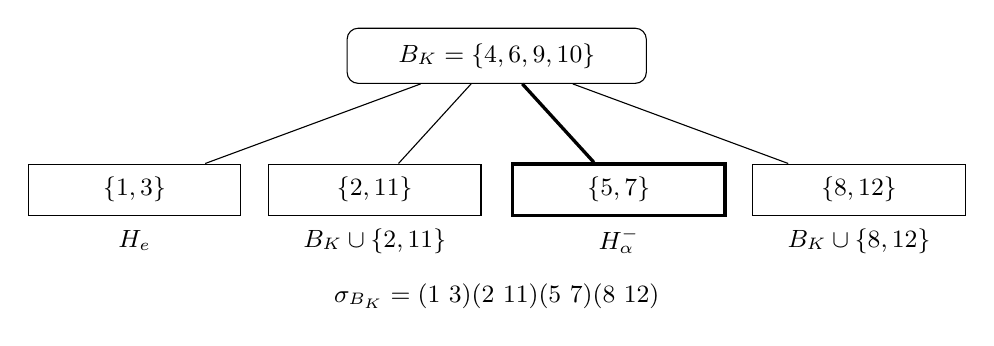
\begin{tikzpicture}[x=1cm,y=1cm, every node/.style={font=\small}]
 \node[draw,rounded corners,minimum width=3.8cm,minimum height=.7cm]
  (b) at (0,0) {$B_K=\{4,6,9,10\}$};
 \node[draw,minimum width=2.7cm,minimum height=.65cm]
  (p1) at (-4.6,-1.7) {$\{1,3\}$};
 \node[draw,minimum width=2.7cm,minimum height=.65cm]
  (p2) at (-1.55,-1.7) {$\{2,11\}$};
 \node[draw,very thick,minimum width=2.7cm,minimum height=.65cm]
  (p3) at (1.55,-1.7) {$\{5,7\}$};
 \node[draw,minimum width=2.7cm,minimum height=.65cm]
  (p4) at (4.6,-1.7) {$\{8,12\}$};
 \draw (b) -- (p1); \draw (b) -- (p2);
 \draw[very thick] (b) -- (p3); \draw (b) -- (p4);
 \node at (-4.6,-2.35) {$H_e$};
 \node at (-1.55,-2.35) {$B_K\cup\{2,11\}$};
 \node at (1.55,-2.35) {$H^-_\alpha$};
 \node at (4.6,-2.35) {$B_K\cup\{8,12\}$};
 \node at (0,-3.05)
  {$\sigma_{B_K}=(1\ 3)(2\ 11)(5\ 7)(8\ 12)$};
\end{tikzpicture}
\caption{The concrete star of the dodecaphasic flag. Each line
indicates the union of the central four-element set with the pair at its endpoint; the
thick line marks the hexad also selected by the signs
preceding the carry of $\alpha$. The four pairs exhaust the eight
outer positions.}
\label{exc:fig-estrella}
\end{figure}

\begin{proposition}[The family of stars]
\label{exc:m12}
The $\binom{12}4=495$ permutations $\sigma_B$ preserve $\mathcal H$.
The group they generate has order $95040$ and is the Mathieu group
$M_{12}$ in its action on the small Witt design.
\end{proposition}

\begin{proof}
Preservation is a finite check on the
$132$ hexads of \eqref{exc:codigo}: for each four-element set, the
four petals are constructed and one verifies
$\{\sigma_B(H):H\in\mathcal H\}=\mathcal H$.
Closure under composition of these permutations produces $95040$
elements. In lexicographic enumeration, it suffices to successively add
six stars not yet contained in the group; the intermediate orders
are $2,6,18,360,7920,95040$, and the $495$ stars belong to the
final group. The procedure and the six generators are made explicit in
the provenance technical note. Finally, one applies the recognition
of the automorphism group of $S(5,6,12)$ as $M_{12}$, whose order is
$12\cdot11\cdot10\cdot9\cdot8=95040$.
\end{proof}

An individual star generates a cyclic group of order two. It does not
by itself generate $M_{12}$, much less the Monster. Nor does the
existence of $495$ generators of a permutation group prove that
each is the transport of a specific TPK loop. That assertion
requires the corresponding loop map; the result established here
is the finite incidence action.

\begin{remark}[Equality of traces does not identify operators]
On $V_{11}$, a star has spectrum $+1$ with multiplicity seven
and $-1$ with multiplicity four. Its normalized trace is $3/11$.
A rank-three projector on the same space also has normalized trace
$3/11$, but spectrum $1^3,0^8$. They are not conjugate: their
minimal polynomials and spectra differ. The intertwiner
\eqref{exc:incidencia} transports defined operators; it does not turn
this scalar coincidence into an equivalence of operators.
\end{remark}

\subsection{The binary residue and the five regions of \texorpdfstring{$\pi$}{pi}}
\label{exc:cinco-regiones}

The next recognition uses the extended binary Golay
code $G_{24}$, with parameters $[24,12,8]_2$. Its weights are
$0,8,12,16,24$, and the weight-eight supports form the design
$S(5,8,24)$. Fix a dodecad $D$, the support of a word of weight
twelve. This datum and the incidence isomorphism to be declared
below belong to the realization chart; they are not used to
generate or select the decimals of $\pi$.

\begin{proposition}[Residue of a dodecad and lifting of hexads]
\label{exc:residuo-binario}
The set
\[
 \mathcal H(D)=
 \{O\cap D: O\text{ is an octad},\ |O\cap D|=6\}
\]
is an $S(5,6,12)$ system on $D$. Each of its hexads has
a unique lift to an octad. For any four-element set $B\subset D$,
the five octads containing it split into four residual
lifts and a unique octad $O_B^\perp$ with $O_B^\perp\cap D=B$.
\end{proposition}

\begin{proof}
A five-element set $A\subset D$ belongs to a unique octad $O$. If
$j=|O\cap D|$, the binary word given by the sum of $O$ and $D$ has weight
$20-2j$. Among the allowed weights, and with $0\leq j\leq8$, only
$j=2,4,6$ are possible. Since $A\subset O\cap D$, we have $j\geq5$
and therefore $j=6$. This gives existence and uniqueness of the residual
hexad, as well as uniqueness of its lift by choosing five of its
points. Moreover,
\[
 \lambda_4(S(5,8,24))=\frac{\binom{20}1}{\binom41}=5,
 \qquad
 \lambda_4(S(5,6,12))=4.
\]
The four residual hexads over $B$ give four distinct octads.
The fifth cannot meet $D$ in six points, since it would give another residual
hexad; because it contains $B$, its intersection has size four and
equals $B$.
\end{proof}

A chart $\ell:[12]\to D$ preserving hexads identifies
$\mathcal H$ with $\mathcal H(D)$. Its existence is the recognition
of the design already constructed as the small Witt design; a concrete
choice of $\ell$ fixes the relabeling. The lift
\[
 \iota_D:\mathcal H\longrightarrow
       \{\text{octads of }G_{24}\},
 \qquad H\longmapsto O\text{ such that }O\cap D=\ell(H),
\]
is injective because intersection with $D$ recovers $\ell(H)$.
This injectivity has hexads as its domain, not the register $K$.

The relation to the five regions of $\pi$ preserves richer data
than the number five. The emissions and their signatures are:
\begin{center}
\small
\begin{tabular}{@{}crll@{}}
\toprule
Region & Multiplicity & Emission $U_6$ & Signature \\
\midrule
$\perp$ & $432$ & $(501,614,498,169,272,272)$ & $555555$ \\
$++_1$ & $144$ & $(810,923,870,169,272,272)$ & $339555$ \\
$++_2$ & $144$ & $(810,983,810,169,272,272)$ & $393555$ \\
$++_3$ & $144$ & $(870,923,810,169,272,272)$ & $933555$ \\
$--$ & $144$ & $(870,923,810,418,674,521)$ & $933717$ \\
\bottomrule
\end{tabular}
\end{center}
In each three-digit decimal block, the signature uses the modular
difference of the first two digits. The five emissions have the
same visible trit word $w_\pi=010211$, but not the same
regional genealogy. The three positive regions preserve the tail
$169|272|272$; the negative region changes it to $418|674|521$;
the transverse region has constant signature and greater multiplicity.

The marked extension of the regional chart sends the transverse region
to $O_{\ell(B_K)}^\perp$, the negative one to $\iota_D(H^-_\alpha)$, and the
three positive ones to the other three lifts of the star. This
realizes the $4+1$ partition of the five octads over $\ell(B_K)$.
The individual correspondence between the three positive names and
the three remaining petals requires a chart ordering; incidence
does not determine it without that datum. Thus the precise assertion is a
marked correspondence of regions, compatible with their roles and the
flag, not a canonical bijection deduced from cardinality five.

The identity $432+4\cdot144=1008$ preserves the regional
multiplicities. Also, $1008=36\cdot28$, and an octad has
$\binom82=28$ pairs. These equalities are arithmetic catalogue
checks, not substitutes for the map $\iota_D$ or the regional chart.

\input{sections/estrella_pentadica_recuperada.tex}

\subsection{From the ternary code to the Niemeier lattice}
\label{exc:niemeier}

The passage to dimension twenty-four need not first go through the
binary code. It is performed directly from $C_W$ by discriminant
gluing. Two compatible prolongations are thus distinguished:
one preserves the residue $W_{12}\subset W_{24}$; the other constructs the
lattice on which the vertex operator algebra will be realized.

Let $A_2=\mathbb Z a_1\oplus\mathbb Z a_2$ have Gram matrix
\[
 \begin{pmatrix}2&-1\\-1&2\end{pmatrix},
 \qquad \rho=a_1+a_2,\qquad \rho^2=2.
\]
We represent the three classes of $A_2^*/A_2$ by
\[
 \varpi_0=0,\qquad
 \varpi_1=\frac{2a_1+a_2}{3},\qquad
 \varpi_2=\frac{a_1+2a_2}{3}.
\]
The map $j\mapsto\varpi_j+A_2$ additively identifies
$\mathbb F_3$ with that discriminant group. For $c\in C_W$, write
$\phi(c)=(\varpi_{c_1},\ldots,\varpi_{c_{12}})$ and define
\begin{equation}
 N(C_W)=\bigcup_{c\in C_W}\bigl(A_2^{12}+\phi(c)\bigr).
 \label{exc:niemeier-def}
\end{equation}

\begin{theorem}[Ternary gluing]
\label{exc:niemeier-teorema}
The object \eqref{exc:niemeier-def} is a positive, even,
unimodular lattice of rank $24$. Its root system is exactly
$A_2^{12}$; it is therefore recognized as the Niemeier lattice with
that root system.
\end{theorem}

\begin{proof}
Linearity of the code makes the union of classes closed under
addition. Self-orthogonality annihilates the discriminant pairing:
this is a multiple of $c\cdot d/3$ modulo $\mathbb Z$. Thus the
lattice is integral. The norm of a glue class is
$2\operatorname{wt}(c)/3$ modulo $2\mathbb Z$. The weights in
\eqref{exc:enumerador} are multiples of three, so it is even.

The index of $A_2^{12}$ in $N(C_W)$ is $|C_W|=3^6$. Consequently,
\[
 \det N(C_W)=\frac{3^{12}}{(3^6)^2}=1.
\]
Positivity comes from the orthogonal sum of the twelve $A_2$ metrics.
In a nonzero class of $A_2^*/A_2$, the minimum norm is $2/3$;
every nonzero word has at least six nonzero positions.
Thus a vector in a nontrivial glue class has norm
at least $6\cdot2/3=4$. No roots of norm two occur outside
$A_2^{12}$. Within it, the roots are precisely those of its
twelve components.
\end{proof}

\subsection{Incidence selection of the rootless unimodular neighbor}
\label{exc:leech}

\input{sections/incidencia_reticulo.tex}

The flag label $o_*=1$ is now realized as one of the
twelve $A_2$ components. This operation declares the preceding metric and
the positive radial chamber
\[
 v(a)=\sum_{i=1}^{12}a_i\rho_i,
 \qquad a_i=1+3b_i,\quad b_i\in\mathbb Z_{\geq0}.
\]
The evenness requirement for the index-three neighbor is
$v(a)^2\equiv0\pmod{18}$. Since
\[
 v(a)^2=2\sum_i(1+3b_i)^2,
\]
this congruence is equivalent to $\sum_i b_i\equiv1\pmod3$. The smallest
norm in the chamber is attained with a single $b_i=1$ and
all others zero; it is $54$. The marked origin selects
\begin{equation}
 v_\alpha=4\rho_1+\rho_2+\cdots+\rho_{12},
 \qquad v_\alpha^2=54.
 \label{exc:vector}
\end{equation}
The word ``smallest'' refers to this positive chamber. It does not assert
minimality throughout the residue class: the vector
$(a_1-2a_2,\rho,\ldots,\rho)$ represents the same class modulo three
and has norm $14+11\cdot2=36$. The chamber restriction is part
of the construction data, not a conclusion that can be omitted.

Let $N=N(C_W)$. Define
\begin{equation}
 N_{\alpha,0}=\{x\in N:\langle x,v_\alpha\rangle\equiv0\pmod3\},
 \qquad
 N_\alpha=N_{\alpha,0}+\mathbb Z\frac{v_\alpha}{3}.
 \label{exc:vecino}
\end{equation}

\begin{theorem}[Leech neighbor determined by the marked flag]
\label{exc:teorema-leech}
With the declared metric and chamber, $N_\alpha$ is a positive,
even, unimodular lattice of rank $24$, with no vectors of norm two.
By the corresponding classification theorem, it is isometric to the
Leech lattice $\Lambda_{24}$.
\end{theorem}

\begin{proof}
The character $x\mapsto\langle x,v_\alpha\rangle\bmod3$ is nonzero:
a simple root of a component pairs with $a_i\rho_i$ to give
$a_i\equiv1\pmod3$. Hence $[N:N_{\alpha,0}]=3$ and
$\det N_{\alpha,0}=9$. Moreover,
$v_\alpha/3\in N_{\alpha,0}^*$ and $v_\alpha\in N_{\alpha,0}$.
If $v_\alpha/3$ belonged to $N$, integrality of $N$ would make
all pairings with $v_\alpha$ divisible by three,
contradicting the nonzero character. The class of $v_\alpha/3$ therefore
has order three. It follows that
\[
 [N_\alpha:N_{\alpha,0}]=3,
 \qquad \det N_\alpha=9/3^2=1.
\]
The extension is integral, and for $x\in N_{\alpha,0}$,
\[
 \left(x+m\frac{v_\alpha}{3}\right)^2
   =x^2+2m\frac{\langle x,v_\alpha\rangle}{3}+6m^2
   \in2\mathbb Z.
\]
It is therefore even.

It remains to exclude roots, which is the decisive step. The roots of $N$
belong to $A_2^{12}$. Their pairings with $v_\alpha$ are
congruent to $\pm1$ or $\pm2$ modulo three; none belongs to
$N_{\alpha,0}$. For the other two classes of the neighbor, each component
belongs to one of the local classes
\[
 A_2+\varpi_j\pm\rho/3,\qquad j=0,1,2.
\]
Since $4\rho/3\equiv\rho/3\pmod{A_2}$, this description also
holds in the distinguished component. Writing a local vector
as $(u a_1+v a_2)/3$, its norm is
$2(u^2-uv+v^2)/9$. The six preceding classes have nonzero
residues and minimum $2/9$: representatives minimizing the quadratic form
are $(\pm1,0),(0,\pm1),(1,1),(-1,-1)$ in the appropriate residues.
A vector in a new class therefore has norm at least
$12\cdot2/9=8/3>2$. There are no roots in any of the three classes.
The classification of positive even unimodular lattices of
rank twenty-four identifies the unique rootless case with
$\Lambda_{24}$.
\end{proof}

The argument does not recognize Leech from a coincidence of dimension.
It constructs the gluing, proves integrality, evenness, and determinant, and
eliminates roots by a local bound. Only then does it apply the
classification theorem. Dependence on $\alpha$ is preserved in
the flag selecting $o_*$ and in the vector \eqref{exc:vector};
the scalar value of the constant is not converted into a lattice
length.

\subsection{The vertex operator algebra and the Monster}
\label{exc:voa}

Let $\Lambda=N_\alpha$, already recognized as Leech. The next step
uses its integral lattice, not a decimal expansion. The
lattice vertex operator algebra construction is written
\[
 V_\Lambda=M(1)\otimes\mathbb C_\varepsilon[\Lambda].
\]
Here $M(1)$ is the rank-twenty-four Heisenberg oscillator
space; $\mathbb C_\varepsilon[\Lambda]$ is the group algebra
twisted by the cocycle of the lattice central extension. The
cocycle and the lifting of isometries are part of the
construction: a bare vector-space sum does not determine the vertex
products.

Negation $\lambda\mapsto-\lambda$ admits the standard lift
$\theta$. With its twisted module and the compatible parity choice,
the Frenkel--Lepowsky--Meurman construction produces
\begin{equation}
 V^\natural_{\rm HMT}
   =V_\Lambda^+\oplus(V_\Lambda^T)^+.
 \label{exc:flm}
\end{equation}
The sign $+$ denotes the even part of the lifted action. The expression
includes the orbifold vertex product; it is not merely a sum
of graded spaces.

\begin{theorem}[Prolongation to the Moonshine module]
\label{exc:moonshine}
The algebra \eqref{exc:flm}, constructed on the neighbor
\eqref{exc:vecino}, is a realization of the Moonshine algebra
$V^\natural$. It has central charge $24$, zero weight-one component,
and automorphism group isomorphic to the Monster $\mathbb M$. Its graded
character is
\begin{equation}
 \operatorname{Tr}_{V^\natural_{\rm HMT}}q^{L_0-1}
   =J(\tau)=j(\tau)-744
   =q^{-1}+196884q+21493760q^2+\cdots,
 \qquad q=e^{2\pi i\tau}.
 \label{exc:j}
\end{equation}
\end{theorem}

\begin{proof}
Theorem \ref{exc:teorema-leech} verifies the lattice hypotheses:
positivity, evenness, unimodularity, rank twenty-four, and absence of
roots. One then applies the Frenkel--Lepowsky--Meurman
construction and theorem for the Leech lattice. These identify
the orbifold with $V^\natural$ and establish its character and automorphism
group. Composing the flag, the neighbor, and the VOA
construction functor gives the realization stated here. The group is not
deduced from the coefficient $196884$.
\end{proof}

The theorem used is a subsequent classical recognition with
verified hypotheses, not a new proof in this article of the
FLM construction \cite{flm}.
Furthermore, the notation $q=e^{2\pi i\tau}$ is the conventional Fourier
variable used to recognize the character. It introduces neither $\pi$
nor $e$ as inputs to the coinductive generator that has already determined them.

Part of the trace mechanism can be seen before the orbifold.
Only the zero lattice vector is fixed by negation; each
oscillator contributes alternating sign. Hence
\[
 \operatorname{Tr}_{V_\Lambda}\theta q^{L_0-1}
   =t_2(\tau)
   :=q^{-1}\prod_{n\geq1}(1+q^n)^{-24}.
\]
This trace in the lattice algebra must not be confused with the
character without insertion of $V^\natural$. Nor does it by itself identify
a Monster conjugacy class: the space, insertion,
and lift must be specified before functions are compared.

\input{sections/incidencia_automorfismos.tex}

\subsection{Graded Moonshine traces and the Monster representation}
\label{exc:alcance}

For $g\in\operatorname{Aut}(V^\natural_{\rm HMT})$, the trace
with insertion is
\[
 T_g(\tau)=
 \operatorname{Tr}_{V^\natural_{\rm HMT}}gq^{L_0-1}.
\]
The monstrous Moonshine theorem identifies these series as
Hauptmoduln of the corresponding genus-zero groups
\cite[Theorem~1.1]{borcherds}.
The character $J$, the group $\mathbb M$, and the family $g\mapsto T_g$
are realizations of the algebra already constructed. They do not form a causal
sequence in which $J$ is first guessed and the Monster then deduced.

The unit has a precise algebraic location here. The weight-zero
subspace is the vacuum line, \(V^\natural_0=\CC\mathbf1\), and
the coefficient of \(q^{-1}\) in \(J\) is therefore \(1\). In weight one,
the dimension is zero, accounting for the absence of the constant term
in \(J=j-744\). A vertex algebra morphism preserves the vacuum
vector. This property supplies the technical meaning of preservation
of the unit at this level; the unit of the cylindrical observables
is preserved by the precomposition proved earlier. The relation
between the two levels must follow the construction maps with their units.

In weight two, the equality
\[
 196884=1+196883=196560+324=54(5\cdot729+1).
\]
appears.
The first decomposition corresponds to the trivial conformal line and the
irreducible component of dimension $196883$ of the Monster
representation. The other expressions have lattice or arithmetic
readouts. Their equality does not automatically identify their summands
with regions, words, or TPK routes. Doing so would require
presenting the maps between those spaces and proving that they respect the
relevant actions.


In particular, an isometry $N_\alpha\simeq\Lambda_{24}$ induces
a realization of \eqref{exc:flm}, and a choice of isomorphism
with $V^\natural$ transports its automorphism group. This has not
constructed a Monster action on the digits of
$\pi$, on the blocks of $K$, or on all TPK histories.
Such an additional assertion would require a representation
$\rho_{\rm TPK}$ and a map $F$ with an explicit square
\[
 F\rho_{\rm TPK}(g)=\rho_{V^\natural}(g)F,
\]
including domain, codomain, and preserved information. The absence
of that step from the present assertion does not withdraw the incidence
intertwiner $U_W$, the flag, or the neighbor already constructed; it only
delimits a different strengthening, concerning action on the source state.

The chain established in this section can be summarized, keeping
its transport data visible, as
\begin{align*}
 &\text{APP--TRIT--TPK and arithmetic state with trajectory memory}
   \longrightarrow (w_j,f_j;K,Z_0)\\
 &\longrightarrow (C_W,\mathcal H;B_K\subset H^-_\alpha,
                   P_\pi,H_e,H_\varphi,H_{\rm APP})\\
 &\longrightarrow \bigl(N(C_W),o_*,\text{metric and chamber}\bigr)
   \longrightarrow N_\alpha
   \longrightarrow V^\natural_{\rm HMT}.
\end{align*}
At the incidence level, the stars generate $M_{12}$ and the
residual chart realizes the regional $4+1$ structure in $W_{24}$.
At the lattice and VOA level, the construction gives Leech and the
Moonshine module. These are prolongations of the same marked source, with
different objects and maps. Causal continuity does not require
identifying their codomains or erasing the explicit choices
of frame, chamber, and lift.

The result of the section is therefore a consolidated derivation:
the finite and lattice proofs make effective the passage from
dodecaphasic incidence to the hypotheses of the recognition
theorems. This result concerns the specified constructions and
hypotheses; it does not add experimental validation to the
comparison of constants.
